\documentclass[t, aspectratio=169]{beamer}
\usepackage[utf8]{inputenc}
\usepackage[T1]{fontenc}
\usepackage{amsthm,amsmath,amssymb}
\usepackage{tabularx}
\usepackage{booktabs}
\usepackage{array}
\usepackage[table]{xcolor}
\usepackage{lmodern}
\usepackage{graphicx}
\usepackage{tikz}
\usetikzlibrary{shapes.geometric, arrows.meta, positioning, calc}

% --- FONT SIZES ---
\setbeamerfont{frametitle}{size=\large}

% --- TIKZ STYLES ---
\tikzset{
    block_pink/.style={rectangle, draw, rounded corners, fill=pink!20, text width=3.5cm, text centered, minimum height=1.2cm},
    block_yellow/.style={rectangle, draw, rounded corners, fill=yellow!20, text width=3.5cm, text centered, minimum height=1.2cm},
    block_green/.style={rectangle, draw, rounded corners, fill=green!20, text width=3.5cm, text centered, minimum height=1.2cm},
    block_blue/.style={rectangle, draw, rounded corners, fill=blue!10, text width=3.5cm, text centered, minimum height=1.2cm},
    arrow/.style={-Latex, thick}
}

% --- MARGIN CONFIGURATION ---
\def\slideContentLeftMargin{0.5cm} 
\def\slideContentRightMargin{1cm}   
\def\hustHeaderHeight{1cm}        
\def\slideContentBotMargin{3.5cm}   

\usepackage[blue, 169]{beamerthemeHUST} 

\renewcommand{\titlePageTitleX}{-0.5cm}
\renewcommand{\titlePageTitleY}{-0.5cm}
\renewcommand{\hustTitleAlign}{\alignLeft} 
\renewcommand{\hustSubtitleAlign}{\alignLeft}
\renewcommand{\hustAuthorAlign}{\alignLeft}
\renewcommand{\hustInstAlign}{\alignLeft}

\title{ZERO-LATENCY HARDWARE-ALGORITHM CO-DESIGNED ADAPTIVE RECONCILIATION FOR QKD}
\subtitle{A Syndrome-Based Statistical Controller Architecture}
\author{Nguyen Minh Sang, Vu Quang Huy} 
\institute{Research Proposal}

\begin{document}
	
	% Title page
	\husttitlepage
	
	\begin{frame}[allowframebreaks]{Table of Contents}
		\tableofcontents[hideallsubsections]
	\end{frame}
	
	\resetPageCount  
	\showPageNumber  
	
	\useStyleHustFull
	\useThinBar 
	
	% =================================================================
	\section{Overview \& Objectives}
	% =================================================================
	
	\begin{frame}{Research Context: FSO QKD Networks}
        \textbf{The Challenge of Satellite QKD:}
        \begin{itemize}
            \item \textbf{Free-Space Optical (FSO) Channels:} Suffer from intense atmospheric turbulence, causing Quantum Bit Error Rate (QBER) to fluctuate wildly within milliseconds.
            \vspace{0.8em}
            \item \textbf{The Parameter Estimation Dilemma:} Traditional QKD sacrifices $\sim 10\%$ of raw keys to estimate QBER. In FSO, this estimation becomes obsolete instantly due to rapid channel changes.
            \vspace{0.8em}
            \item \textbf{The Standard Solution:} \textit{Blind Reconciliation} is used to dynamically adapt Code Rates without sacrificing key bits, but it introduces fatal system bottlenecks.
        \end{itemize}
	\end{frame}
    	\begin{frame}{System Overview Diagram}
        \textbf{Post Processing Architecture}
        \begin{center}
            % Vui lòng lưu bức ảnh bạn vừa gửi với tên 'system_diagram.png' vào cùng thư mục với file Slide_HUST_Direction.tex
            \includegraphics[height=0.75\textheight]{Screenshot 2026-08-08 153742.png}
        \end{center}
	\end{frame}

	\begin{frame}{Project Objectives}
        \textbf{Core Innovations:}
        \begin{itemize}
            \item \textbf{Algorithmic Breakthrough:} Prove that \textit{Syndrome Hamming Weight (SHW)} is a sufficient statistical bound for QBER estimation, eliminating trial-and-error ping-pong protocols.
            \vspace{0.8em}
            \item \textbf{Hardware Architecture:} Design a \textit{Hardware Statistical Controller} that acts as an autonomous on-chip brain to dynamically reconfigure the LDPC datapath in $O(1)$ clock cycles.
            \vspace{0.8em}
            \item \textbf{Cross-Layer Optimization:} Achieve unprecedented Energy-per-bit reductions and Tbps-level latency improvements, challenging current Deep Learning and Blind Reconciliation paradigms.
        \end{itemize}
	\end{frame}
	
	% =================================================================
	\section{Literature Review \& Limitations}
	% =================================================================
	
	\begin{frame}{Literature Review (1/3): Hardware Accelerators}
        \textbf{[1] High-Speed Post-Processing in Continuous-Variable QKD Based on FPGA (2020)}
        \begin{itemize}
            \item \textbf{Achievement:} High-speed CV-QKD post-processing pipeline.
            \item \textcolor{red}{\textbf{Limitation:}} Static hardware. Relies on an external CPU for control, lacking real-time physical layer adaptability to channel fluctuations.
        \end{itemize}
        \vspace{0.8em}
        \textbf{[2] FPGA-based acceleration of QC-LDPC syndrome encoding for QKD (2023)}
        \begin{itemize}
            \item \textbf{Achievement:} High-throughput parallelized syndrome encoding at Alice's side.
            \item \textcolor{red}{\textbf{Limitation:}} Does not solve the decoder-side (Bob) bottleneck where rate-adaptation and iterative decoding power waste actually occur.
        \end{itemize}
	\end{frame}

	\begin{frame}{Literature Review (2/3): Rate-Adaptive Schemes}
        \textbf{[3] A Code Rate-Compatible High-Throughput HW Implementation Scheme (2022)}
        \begin{itemize}
            \item \textbf{Achievement:} FPGA LDPC core supporting multiple Code Rates via puncturing.
            \item \textcolor{red}{\textbf{Limitation:}} Provides the "muscle" but lacks the "brain". Still requires wasteful QBER pre-estimation or slow Blind Ping-Pong protocols to decide \textit{when} to switch rates.
        \end{itemize}
        \vspace{0.8em}
        \textbf{[4] A Collaborative RC QC-LDPC Code Construction Scheme (2024)}
        \begin{itemize}
            \item \textbf{Achievement:} Novel mathematical matrix construction (extension \& splitting) to avoid puncturing degradation.
            \item \textcolor{red}{\textbf{Limitation:}} Pure coding theory. Ignores the severe hardware latency overhead caused by rate-switching during active transmission.
        \end{itemize}
	\end{frame}

	\begin{frame}{Literature Review (3/3): FSO Protocols}
        \textbf{[5] Blind Reconciliation with Protograph LDPC Code Extension for FSO (2024)}
        \begin{itemize}
            \item \textbf{Achievement:} Proposes an elegant blind reconciliation protocol tailored for FSO QKD systems, using a brilliant nested Protograph LDPC matrix construction to facilitate parallel decoding.
            \item \textbf{The Open Hardware Challenge:} While mathematically rigorous, executing the iterative "Blind Ping-Pong" trial-and-error protocol on physical FPGA hardware inevitably introduces latency overheads and dynamic power consumption during failed decoding attempts.
        \end{itemize}
	\end{frame}

	\begin{frame}{The Literature Gap: The "Academic Silo"}
        \textbf{Summary of the Interdisciplinary Gap:}
        \begin{itemize}
            \item \textbf{Coding Theorists (e.g., [4, 5])} design elegant nested matrices and blind protocols but leave the hardware latency and dynamic power overheads as open challenges.
            \item \textbf{VLSI Engineers (e.g., [1, 2])} design ultra-fast decoders but keep them mathematically rigid and passive, unable to autonomously adapt to FSO channel fluctuations.
        \end{itemize}
        \vspace{1em}
        \textbf{\textcolor{blue}{Our Proposed Novelty: Cross-Layer Co-Design}} \\
        We bridge this gap by designing an \textit{Autonomous Hardware Controller}. It inherits the brilliant nested LDPC matrices from recent theoretical works (like [5]), but completely \textbf{bypasses the blind trial-and-error} by using Syndrome Statistical Prediction to select the optimal matrix in one shot.
	\end{frame}

	\begin{frame}{The Blind Reconciliation Bottleneck}
		\begin{center}
		\resizebox{0.6\textwidth}{!}{%
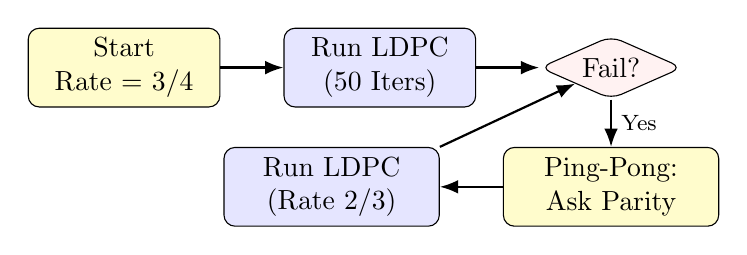
\begin{tikzpicture}[node distance=0.6cm and 0.8cm]

\node (start) [block_yellow,text width=2.2cm,minimum height=1cm]
    {Start\\Rate = 3/4};

\node (decode) [block_blue,right=of start,
    text width=2.2cm,minimum height=1cm]
    {Run LDPC\\(50 Iters)};

\node (check) [block_pink,right=of decode,
    diamond,aspect=2.5,text width=1.2cm,
    minimum height=0.8cm,inner sep=0pt]
    {Fail?};

\node (fail) [block_yellow,below=of check,
    text width=2.5cm,minimum height=1cm]
    {Ping-Pong:\\Ask Parity};

\node (next) [block_blue,left=of fail,
    text width=2.5cm,minimum height=1cm]
    {Run LDPC\\(Rate 2/3)};

% Main flow
\draw[arrow] (start.east) -- (decode.west);
\draw[arrow] (decode.east) -- (check.west);

% Failure branch
\draw[arrow] (check.south) -- node[right]{\footnotesize Yes} (fail.north);

% Horizontal arrow
\draw[arrow] (fail.west) -- (next.east);

% Loop back (không đi xuyên node decode)
\draw[arrow] (next.north east) -- (check.south west);

\end{tikzpicture}
		}
		\end{center}

        \vspace{0.2em}
        \textbf{The Consequence:} 
        \begin{itemize}
            \item To successfully decode a noisy block at Rate 1/2, the FPGA might waste 100 iterations on Rate 3/4 and 2/3 first.
            \item \textcolor{red}{\textbf{Result: $\sim 3\times$ Dynamic Power waste and massive network stalling.}}
        \end{itemize}
	\end{frame}

	% =================================================================
	\section{Our Proposed Solution}
	% =================================================================
	\useStyleLogoOnly 
	\useThickBar      
	\begin{frame}{The "One-Shot Predictive" Protocol}
		\textbf{Hardware-Algorithm Co-Design:}
        \begin{itemize}
            \item We abandon both the slow Blind Ping-Pong and the bloated Deep Learning models.
            \item \textbf{The Core Concept:} The Syndrome is received \textit{once}. A lightweight hardware module instantly calculates its Hamming Weight.
            \item \textbf{Statistical LUT:} Using pre-computed offline Monte-Carlo statistics, a Look-Up Table (LUT) maps the weight directly to the optimal configuration vector.
        \end{itemize}
        
        \vspace{1em}
        \textbf{Advantages:}
        \begin{itemize}
            \item \textbf{Zero-Latency:} Prediction happens in $O(1)$ clock cycles.
            \item \textbf{Ultra-Lightweight:} Consumes $< 1\%$ of FPGA resources compared to AI approaches.
        \end{itemize}
	\end{frame}
	
	\begin{frame}{Autonomous Reconfigurable Architecture}
		\begin{center}
		\resizebox{0.9\textwidth}{!}{%
		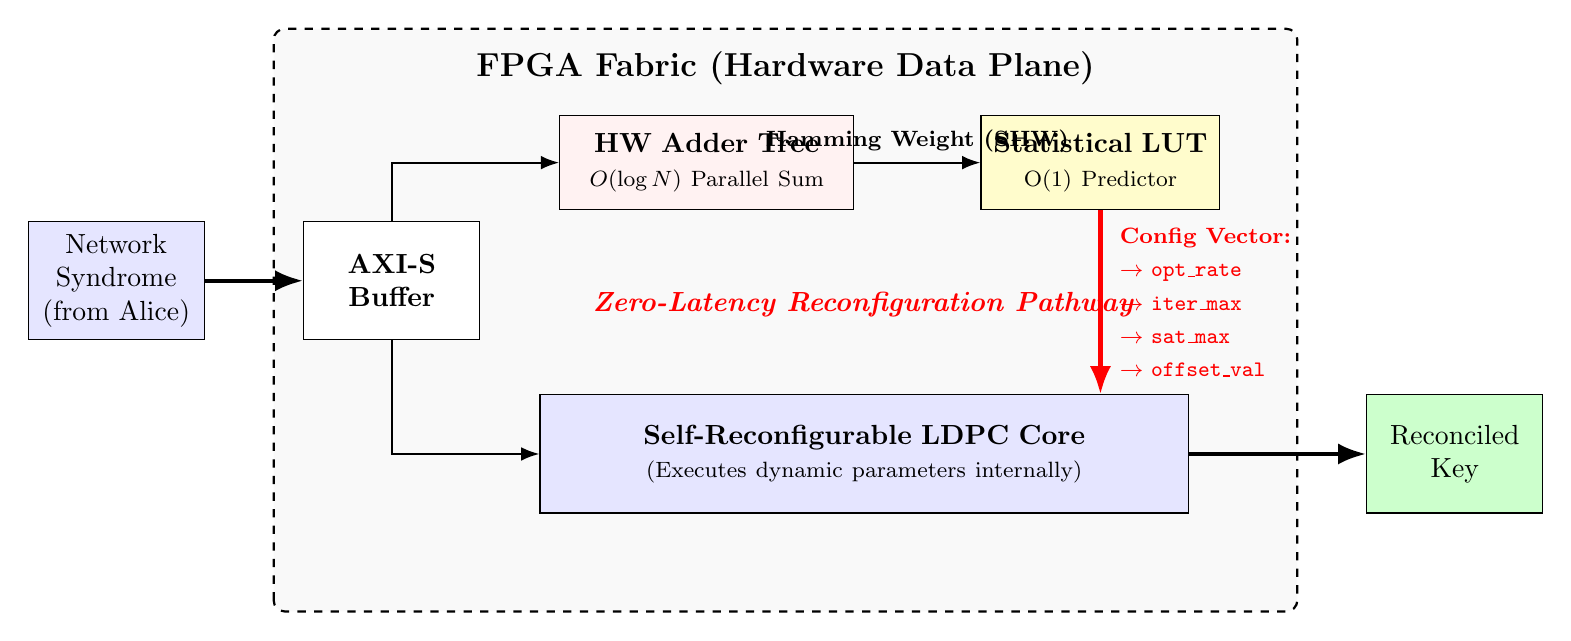
\begin{tikzpicture}
            % FPGA Bounding Box
            \draw[dashed, thick, fill=gray!5, rounded corners] (1, -4.2) rectangle (14, 3.2);
            \node at (7.5, 2.7) [font=\large\bfseries] {FPGA Fabric (Hardware Data Plane)};
            
            % External Input & Output
            \node (input) [rectangle, draw, fill=blue!10, text width=2cm, minimum height=1.5cm, text centered, align=center] at (-1, 0) {Network\\Syndrome\\(from Alice)};
            \node (output) [rectangle, draw, fill=green!20, text width=2cm, minimum height=1.5cm, text centered, align=center] at (16, -2.2) {Reconciled\\Key};
            
            % Internal Nodes
			\node (buffer) [rectangle, draw, fill=white, text width=2cm, minimum height=1.5cm, text centered, align=center] at (2.5, 0) {\textbf{AXI-S\\Buffer}};
            
			\node (adder) [rectangle, draw, fill=pink!20, text width=3.5cm, minimum height=1.2cm, text centered] at (6.5, 1.5) {\textbf{HW Adder Tree}\\ \footnotesize $O(\log N)$ Parallel Sum};
            
			\node (lut) [rectangle, draw, fill=yellow!20, text width=2.8cm, minimum height=1.2cm, text centered] at (11.5, 1.5) {\textbf{Statistical LUT}\\ \footnotesize O(1) Predictor};
            
            \node (ldpc) [rectangle, draw, fill=blue!10, text width=8cm, minimum height=1.5cm, text centered] at (8.5, -2.2) {\textbf{Self-Reconfigurable LDPC Core}\\ \footnotesize (Executes dynamic parameters internally)};
			
            % Connections
			\draw [arrow, ultra thick] (input) -- (buffer);
			\draw [arrow, thick] (buffer) |- (adder);
            \draw [arrow, thick] (buffer) |- (ldpc.west);
			\draw [arrow, thick] (adder) -- node[above, font=\bfseries]{\footnotesize Hamming Weight (SHW)} (lut);
            \draw [arrow, ultra thick] (ldpc) -- (output);
            
            % Control Vector Path
            \draw [arrow, ultra thick, red] (lut.south) -- node[right, align=left, xshift=0.1cm]{\footnotesize \textbf{Config Vector:}\\ \footnotesize $\rightarrow$ \texttt{opt\_rate}\\ \footnotesize $\rightarrow$ \texttt{iter\_max}\\ \footnotesize $\rightarrow$ \texttt{sat\_max}\\ \footnotesize $\rightarrow$ \texttt{offset\_val}} (lut.south |- ldpc.north);
            
            \node at (8.5, -0.3) [font=\bfseries, text=red] {\textit{Zero-Latency Reconfiguration Pathway}};
		\end{tikzpicture}%
		}
		\end{center}
	\end{frame}
	
	\begin{frame}{Mathematical Foundation: Syndrome Weight Analysis}
        \textbf{Why Syndrome Hamming Weight (SHW)?}
        \begin{itemize}\small
            \item The Syndrome $S = H \times E \pmod 2$. Its Hamming Weight is the arithmetic sum: $W_H(S) = \sum_{i=1}^{N} s_i$.
            \item Due to the sparse LDPC matrix (constant column weight $W_c$), we have the bound: $\mathbf{W_H(S) \leq W_c \times W_H(E)}$.
            \item Since $W_H(E)$ is the number of raw errors, $W_H(S)$ serves as a direct linear predictor for QBER.
        \end{itemize}
        
        \vspace{0.2em}
		\begin{center}
		\resizebox{0.5\textwidth}{!}{%
		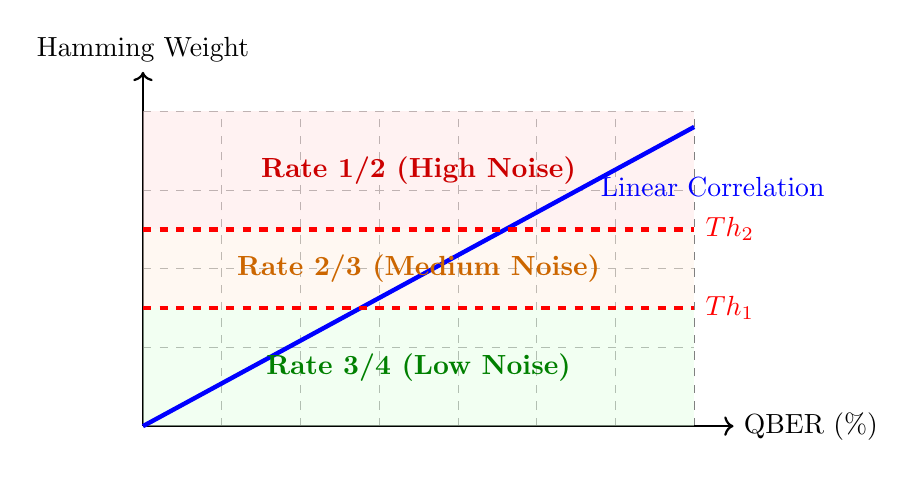
\begin{tikzpicture}
            % Grid and Axes
            \draw[step=1cm,gray,very thin,dashed] (0,0) grid (7,4);
            \draw[->, thick] (0,0) -- (7.5,0) node[right] {QBER (\%)};
            \draw[->, thick] (0,0) -- (0,4.5) node[above] {Hamming Weight};
            
            % Shaded Regions
            \fill[green!10, opacity=0.5] (0,0) rectangle (7,1.5);
            \fill[orange!10, opacity=0.5] (0,1.5) rectangle (7,2.5);
            \fill[red!10, opacity=0.5] (0,2.5) rectangle (7,4);
            
            % Plot Line
            \draw[ultra thick, blue] (0,0) -- (7,3.8) node[pos=0.8, right, xshift=2pt] {Linear Correlation};
            
            % Thresholds
            \draw[ultra thick, red, dashed] (0,1.5) -- (7,1.5) node[right] {$Th_1$};
            \draw[ultra thick, red, dashed] (0,2.5) -- (7,2.5) node[right] {$Th_2$};
            
            % Labels
            \node at (3.5,0.75) [text=green!50!black, font=\bfseries] {Rate 3/4 (Low Noise)};
            \node at (3.5,2.0) [text=orange!80!black, font=\bfseries] {Rate 2/3 (Medium Noise)};
            \node at (3.5,3.25) [text=red!80!black, font=\bfseries] {Rate 1/2 (High Noise)};
		\end{tikzpicture}%
		}
		\end{center}
	\end{frame}

	\begin{frame}{Hardware Implementation: Zero-Latency SHW Extraction}
		\textbf{The Parallel Adder Tree Architecture:}
        \begin{itemize}
            \item To extract the SHW instantly, we deploy a deeply pipelined, highly parallel binary adder tree.
            \item Computes the sum of 1152 bits in $O(\log_2(N))$ stages.
        \end{itemize}
		\begin{center}
		\resizebox{0.6\textwidth}{!}{%
		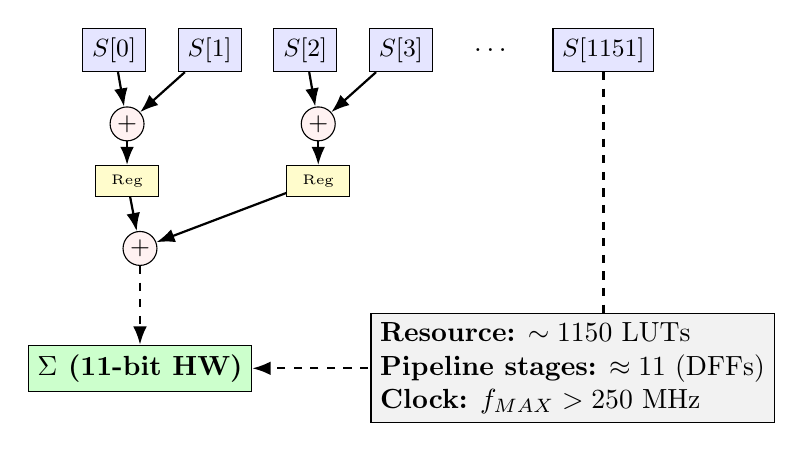
\begin{tikzpicture}[node distance=0.6cm and 0.4cm]
            \tikzstyle{bit}=[rectangle, draw, fill=blue!10, minimum width=0.8cm, font=\small]
            \tikzstyle{adder}=[circle, draw, fill=pink!20, inner sep=1pt, font=\small]
            \tikzstyle{reg}=[rectangle, draw, fill=yellow!20, minimum width=0.8cm, font=\tiny]
            
			\node (in0) [bit] {$S[0]$};
			\node (in1) [bit, right=of in0] {$S[1]$};
			\node (in2) [bit, right=of in1] {$S[2]$};
			\node (in3) [bit, right=of in2] {$S[3]$};
            \node (dots) [right=of in3] {\dots};
			\node (inN) [bit, right=of dots] {$S[1151]$};
            
            % Level 1 Adders
            \node (add1_0) [adder, below right=0.5cm and -0.4cm of in0] {$+$};
            \node (add1_1) [adder, below right=0.5cm and -0.4cm of in2] {$+$};
            \draw [arrow] (in0) -- (add1_0); \draw [arrow] (in1) -- (add1_0);
            \draw [arrow] (in2) -- (add1_1); \draw [arrow] (in3) -- (add1_1);
            
            % Pipeline Reg 1
            \node (r1_0) [reg, below=0.3cm of add1_0] {Reg};
            \node (r1_1) [reg, below=0.3cm of add1_1] {Reg};
            \draw [arrow] (add1_0) -- (r1_0);
            \draw [arrow] (add1_1) -- (r1_1);

            % Level 2 Adders
            \node (add2_0) [adder, below right=0.5cm and -0.4cm of r1_0] {$+$};
            \draw [arrow] (r1_0) -- (add2_0); \draw [arrow] (r1_1) -- (add2_0);

            % Final sum
            \node (sum) [rectangle, draw, fill=green!20, below=1cm of add2_0, font=\bfseries] {$\Sigma$ (11-bit HW)};
            \draw [arrow, dashed, thick] (add2_0) -- (sum);
            \draw [arrow, dashed, thick] (inN) |- (sum);
            
            \node (box) [rectangle, draw, right=1.5cm of sum, align=left, fill=gray!10] {
                \textbf{Resource:} $\sim 1150$ LUTs\\
                \textbf{Pipeline stages:} $\approx 11$ (DFFs)\\
                \textbf{Clock:} $f_{MAX} > 250$ MHz
            };
		\end{tikzpicture}%
		}
		\end{center}
	\end{frame}

	\begin{frame}{Cross-Layer Reconfiguration: The LDPC Datapath}
		\begin{center}
		\resizebox{0.65\textwidth}{!}{%
		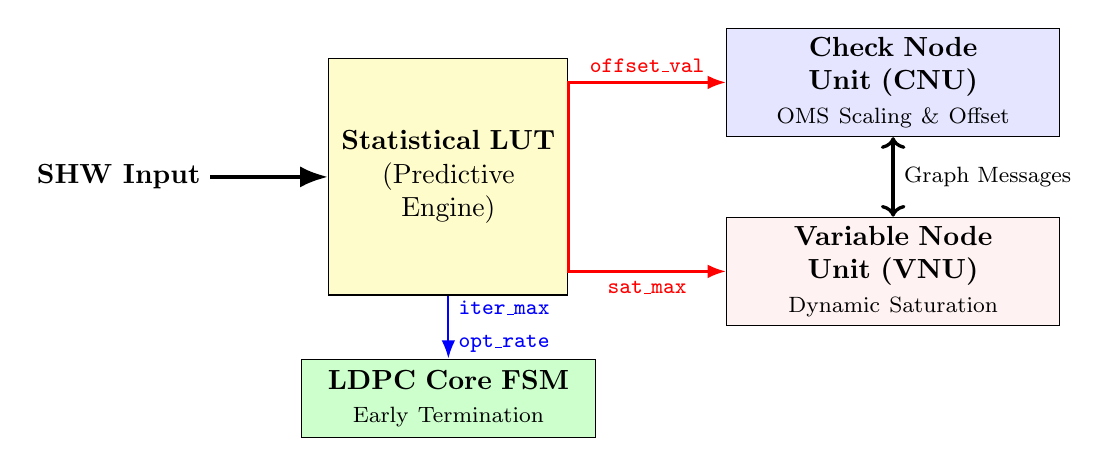
\begin{tikzpicture}[node distance=1.5cm and 1cm]
			\node (lut) [rectangle, draw, fill=yellow!20, text width=2.8cm, text centered, minimum height=3cm] {\textbf{Statistical LUT}\\(Predictive Engine)};
			
            \node (cnu) [rectangle, draw, fill=blue!10, right=2cm of lut, yshift=1.2cm, text width=4cm, text centered, minimum height=1.2cm] {\textbf{Check Node Unit (CNU)}\\ \footnotesize OMS Scaling \& Offset};
            \node (vnu) [rectangle, draw, fill=pink!20, right=2cm of lut, yshift=-1.2cm, text width=4cm, text centered, minimum height=1.2cm] {\textbf{Variable Node Unit (VNU)}\\ \footnotesize Dynamic Saturation};
            \node (fsm) [rectangle, draw, fill=green!20, below=0.8cm of lut, text width=3.5cm, text centered, minimum height=1cm] {\textbf{LDPC Core FSM}\\ \footnotesize Early Termination};

            % Arrows with nice labels
			\draw [arrow, thick, red] (lut.east) |- node[above, near end]{\footnotesize \texttt{offset\_val}} (cnu.west);
            \draw [arrow, thick, red] (lut.east) |- node[below, near end]{\footnotesize \texttt{sat\_max}} (vnu.west);
            \draw [arrow, thick, blue] (lut.south) -- node[right, align=left]{\footnotesize \texttt{iter\_max}\\ \footnotesize \texttt{opt\_rate}} (fsm.north);
            
            \draw [arrow, <->, very thick] (cnu) -- node[right]{\footnotesize Graph Messages} (vnu);
            
            % Input
            \node (shw) [left=1.5cm of lut] {\textbf{SHW Input}};
            \draw [arrow, ultra thick] (shw) -- (lut);
		\end{tikzpicture}%
		}
		\end{center}
        
        \vspace{0.2em}
        \textbf{Real-Time Algorithmic Impact:} 
        \begin{itemize}
            \item \textbf{\texttt{offset\_val}:} Increased dynamically for noisy blocks to break trapping sets.
            \item \textbf{\texttt{sat\_max}:} Limits error-propagation bounds dynamically based on noise density.
            \item \textbf{\texttt{iter\_max}:} Enforces Early Termination to save dynamic power on clean blocks.
        \end{itemize}
	\end{frame}

	\begin{frame}{Cross-Layer Optimization Impacts}
		\begin{itemize}
			\item \textbf{Dynamic Code Rate Selection:} Bypasses blind trial-and-error, jumping straight to the required Rate (1/2, 2/3, or 3/4).
			\item \textbf{Dynamic Power Scaling:} For "easy" blocks, the controller restricts \texttt{iter\_max} to 20 instead of 50, slashing dynamic power consumption.
			\item \textbf{Trapping Set Evasion:} For extremely noisy blocks, the controller proactively alters mathematical parameters (\texttt{sat\_max}, \texttt{offset\_val}) to break topological trapping sets before decoding even begins.
			\item \textbf{Instant Discard:} If QBER $> 6.5\%$, the controller asserts a Discard flag, saving $100\%$ of the energy that would be wasted on a doomed block.
		\end{itemize}
	\end{frame}

    % =================================================================
	\section{Conclusion \& Future Roadmap}
	% =================================================================
	\useStyleHustFull
	\useThinBar 
	
	\begin{frame}{Roadmap to Publication}
		\begin{center}
		\resizebox{0.95\textwidth}{!}{%
		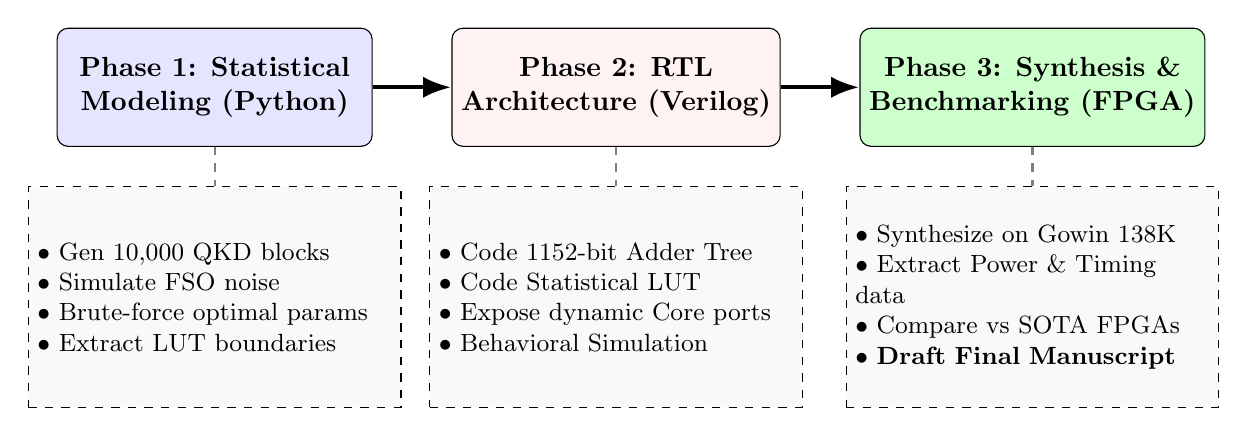
\begin{tikzpicture}[node distance=0.5cm and 0.5cm]
            \tikzstyle{phase}=[rectangle, draw, rounded corners, minimum width=4cm, minimum height=1.5cm, align=center, font=\bfseries]
            \tikzstyle{detail}=[rectangle, draw, dashed, fill=gray!5, text width=4.5cm, minimum height=2.8cm, align=left, font=\small]

            % Phases
            \node (p1) [phase, fill=blue!10] {Phase 1: Statistical\\Modeling (Python)};
            \node (p2) [phase, fill=pink!20, right=1cm of p1] {Phase 2: RTL\\Architecture (Verilog)};
            \node (p3) [phase, fill=green!20, right=1cm of p2] {Phase 3: Synthesis \&\\Benchmarking (FPGA)};

            % Arrows
            \draw [arrow, ultra thick] (p1) -- (p2);
            \draw [arrow, ultra thick] (p2) -- (p3);

            % Details
            \node (d1) [detail, below=0.5cm of p1] {
                $\bullet$ Gen 10,000 QKD blocks\\
                $\bullet$ Simulate FSO noise\\
                $\bullet$ Brute-force optimal params\\
                $\bullet$ Extract LUT boundaries
            };
            
            \node (d2) [detail, below=0.5cm of p2] {
                $\bullet$ Code 1152-bit Adder Tree\\
                $\bullet$ Code Statistical LUT\\
                $\bullet$ Expose dynamic Core ports\\
                $\bullet$ Behavioral Simulation
            };
            
            \node (d3) [detail, below=0.5cm of p3] {
                $\bullet$ Synthesize on Gowin 138K\\
                $\bullet$ Extract Power \& Timing data\\
                $\bullet$ Compare vs SOTA FPGAs\\
                $\bullet$ \textbf{Draft Final Manuscript}
            };
            
            % Connect phases to details
            \draw [dashed, thick, gray] (p1) -- (d1);
            \draw [dashed, thick, gray] (p2) -- (d2);
            \draw [dashed, thick, gray] (p3) -- (d3);
            
		\end{tikzpicture}%
		}
		\end{center}
        
        \vspace{0.5em}
        \begin{itemize}
            \item \textbf{Ultimate Target:} Provide empirical proof of $O(1)$ latency and massive energy reduction, forming the core argument for top-tier IEEE journal submission.
        \end{itemize}
	\end{frame}

	\hustthankyou
	
\end{document}
